\newpage
\section{Hbb HWW and other Channels}
\label{sec:contamination}

Hbb, Hww tagger will also pick up Higgs signals from other channels of Higgs decay. 
In Table~\ref{table:HbbHww}, branching ratio column is taken from standard model Higgs decays at 125GeV. 
For H(ww$\to$qqqq), the branching ratio of W hadronicly decay is already considered. 
Here we assume we have 100000 Standard Model Higgs, and the numbers in the table are showing the number of Higgs pass
the tagger for each channel, with branching ratio taken into account. 
For example, Hcc part, of 100000 SM Higgs,  in Hcc channel, at 1TeV Z' resonance, which is 0.5TeV Higgs, 
we will have 104.42 events pass the Hbb tagger and 102.41 pass the Hww tagger and we also have 82.33 events which fail the 
Hbb tagger but pass the Hww tagger.  

Considering this table, our analysis will move like this way. 
We will keep the Hbb tagger as it was. 
For the Hww channel, we will only select events that fail the Hbb tagger, but pass Hww tagger.
And the effects of this on the background is shown in Fig~\ref{fig:HbbRatio} 


\begin{table}[htbp]
\caption{}
\begin{tabular}{|l|r|r|r|r|}
\hline
1TeV & \multicolumn{1}{l|}{Braching Ratio} & \multicolumn{1}{l|}{Hbb tagger} & \multicolumn{1}{l|}{Pass Hww tagger} & \multicolumn{1}{l|}{Fail Hbb, pass Hww} \\ \hline
Hbb & 57.70 & 11871.78 & 1765.62 & 804.92 \\ \hline
Hww$\to$qqqq & 9.94 & 86.98 & 2416.41 & 2360.75 \\ \hline
Hcc & 3.00 & 104.42 & 102.41 & 82.33 \\ \hline
Htautau & 6.30 & 17.33 & 47.25 & 37.80 \\ \hline
Hgg & 10.00 & 14.99 & 344.83 & 314.84 \\ \hline
 & \multicolumn{1}{l|}{} & \multicolumn{1}{l|}{} & \multicolumn{1}{l|}{} & \multicolumn{1}{l|}{} \\ \hline
1.5TeV & \multicolumn{1}{l|}{Braching Ratio} & \multicolumn{1}{l|}{Hbb tagger} & \multicolumn{1}{l|}{Pass Hww tagger} & \multicolumn{1}{l|}{Fail Hbb, pass Hww} \\ \hline
Hbb & 57.70 & 11444.80 & 1849.29 & 755.87 \\ \hline
Hww$\to$qqqq & 9.94 & 228.62 & 2043.17 & 1916.43 \\ \hline
Hcc & 3.00 & 121.25 & 113.43 & 88.01 \\ \hline
Htautau & 6.30 & 12.60 & 67.10 & 57.02 \\ \hline
Hgg & 10.00 & 69.93 & 244.76 & 174.83 \\ \hline
 & \multicolumn{1}{l|}{} & \multicolumn{1}{l|}{} & \multicolumn{1}{l|}{} & \multicolumn{1}{l|}{} \\ \hline
2TeV & \multicolumn{1}{l|}{Braching Ratio} & \multicolumn{1}{l|}{Hbb tagger} & \multicolumn{1}{l|}{Pass Hww tagger} & \multicolumn{1}{l|}{Fail Hbb, pass Hww} \\ \hline
Hbb & 57.70 & 13816.27 & 1834.86 & 551.04 \\ \hline
Hww$\to$qqqq & 9.94 & 449.29 & 1655.51 & 1435.83 \\ \hline
Hcc & 3.00 & 228.57 & 133.33 & 99.05 \\ \hline
Htautau & 6.30 & 42.21 & 97.34 & 74.66 \\ \hline
Hgg & 10.00 & 157.62 & 315.24 & 262.70 \\ \hline
\end{tabular}
\label{table:HbbHww}
\caption{table of all signals Higgs gen jet pass Hbb tagger, pass Hww tagger, and fail Hbb tagger but pass Hww tagger, assuming we have 100K Higgs decays to all channels.}
\end{table}


\begin{figure}[htb]
\begin{center}
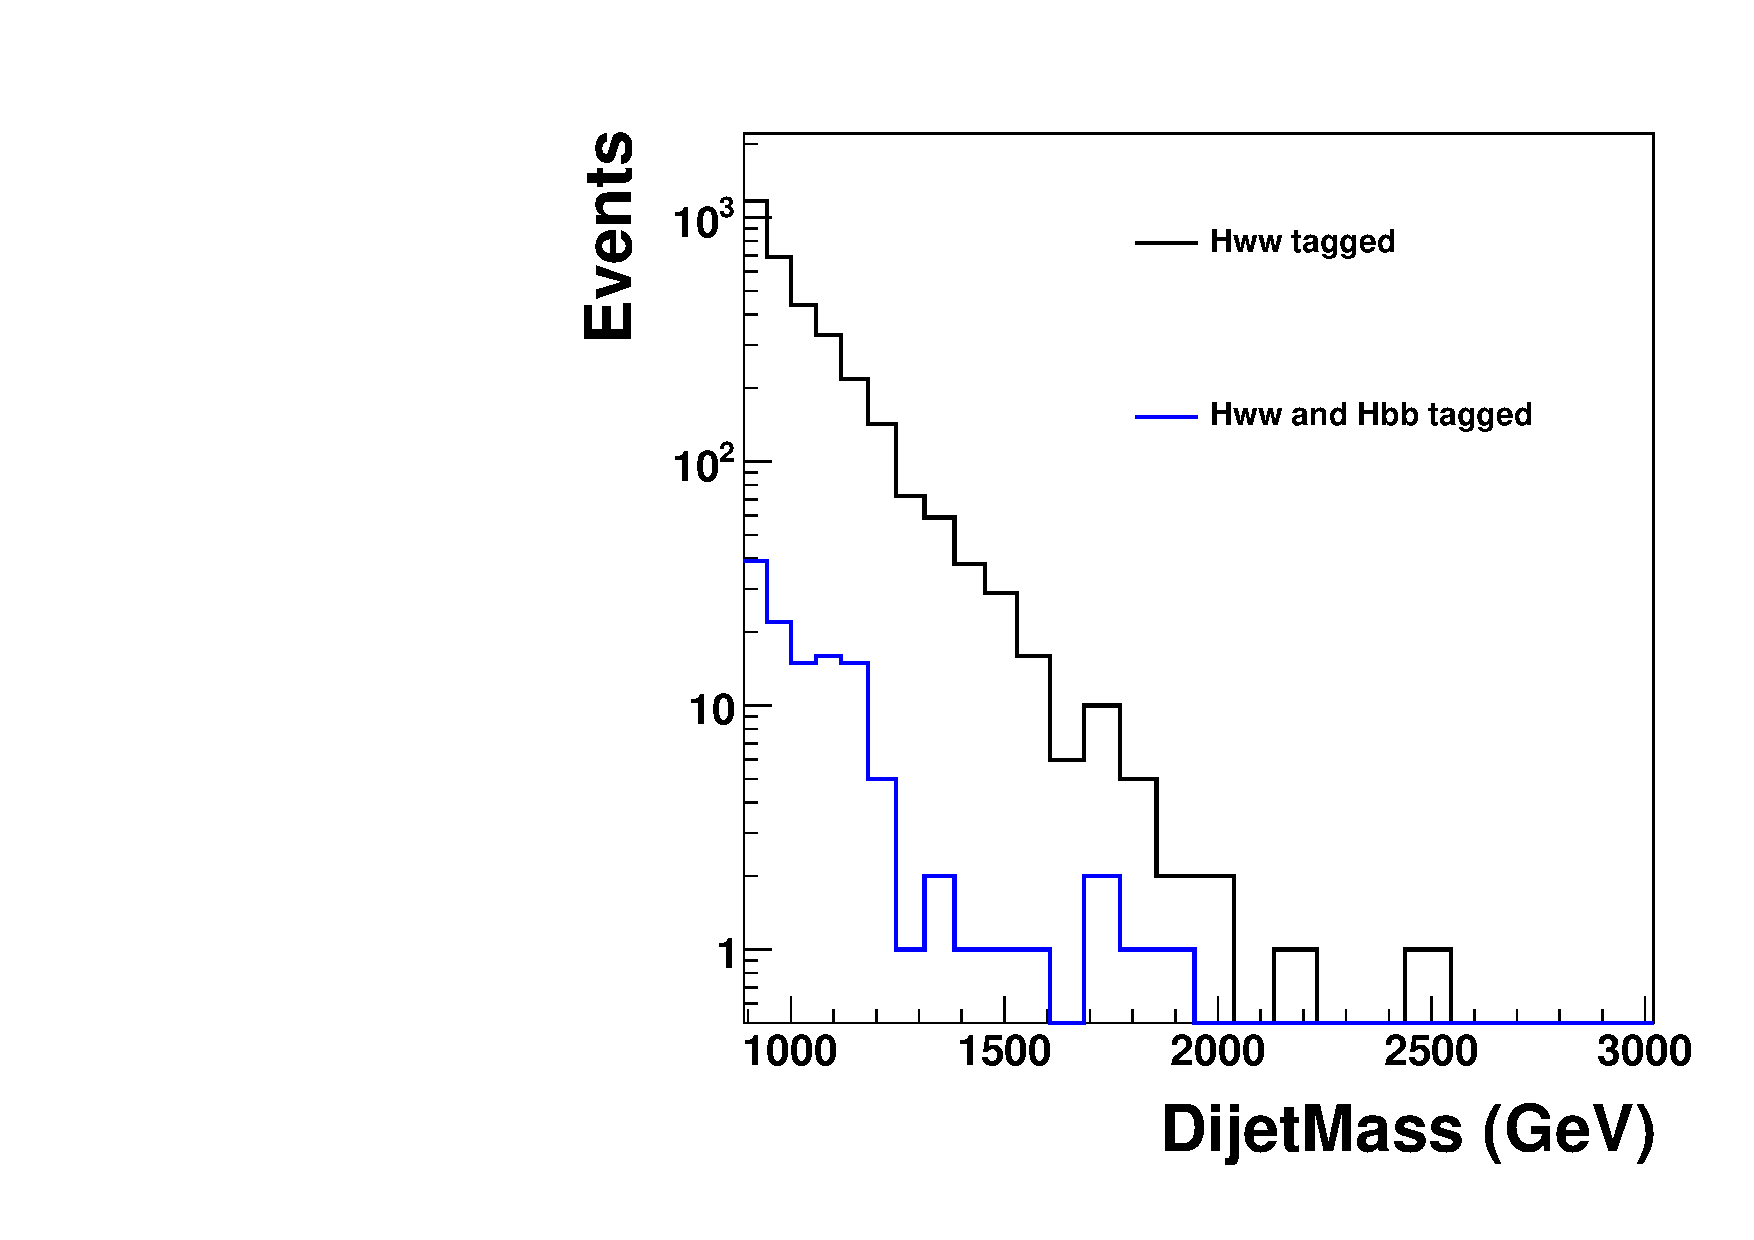
\includegraphics[width=0.49\textwidth]{HqqqqZqqfigs/HbbHww/HighPurity.pdf}
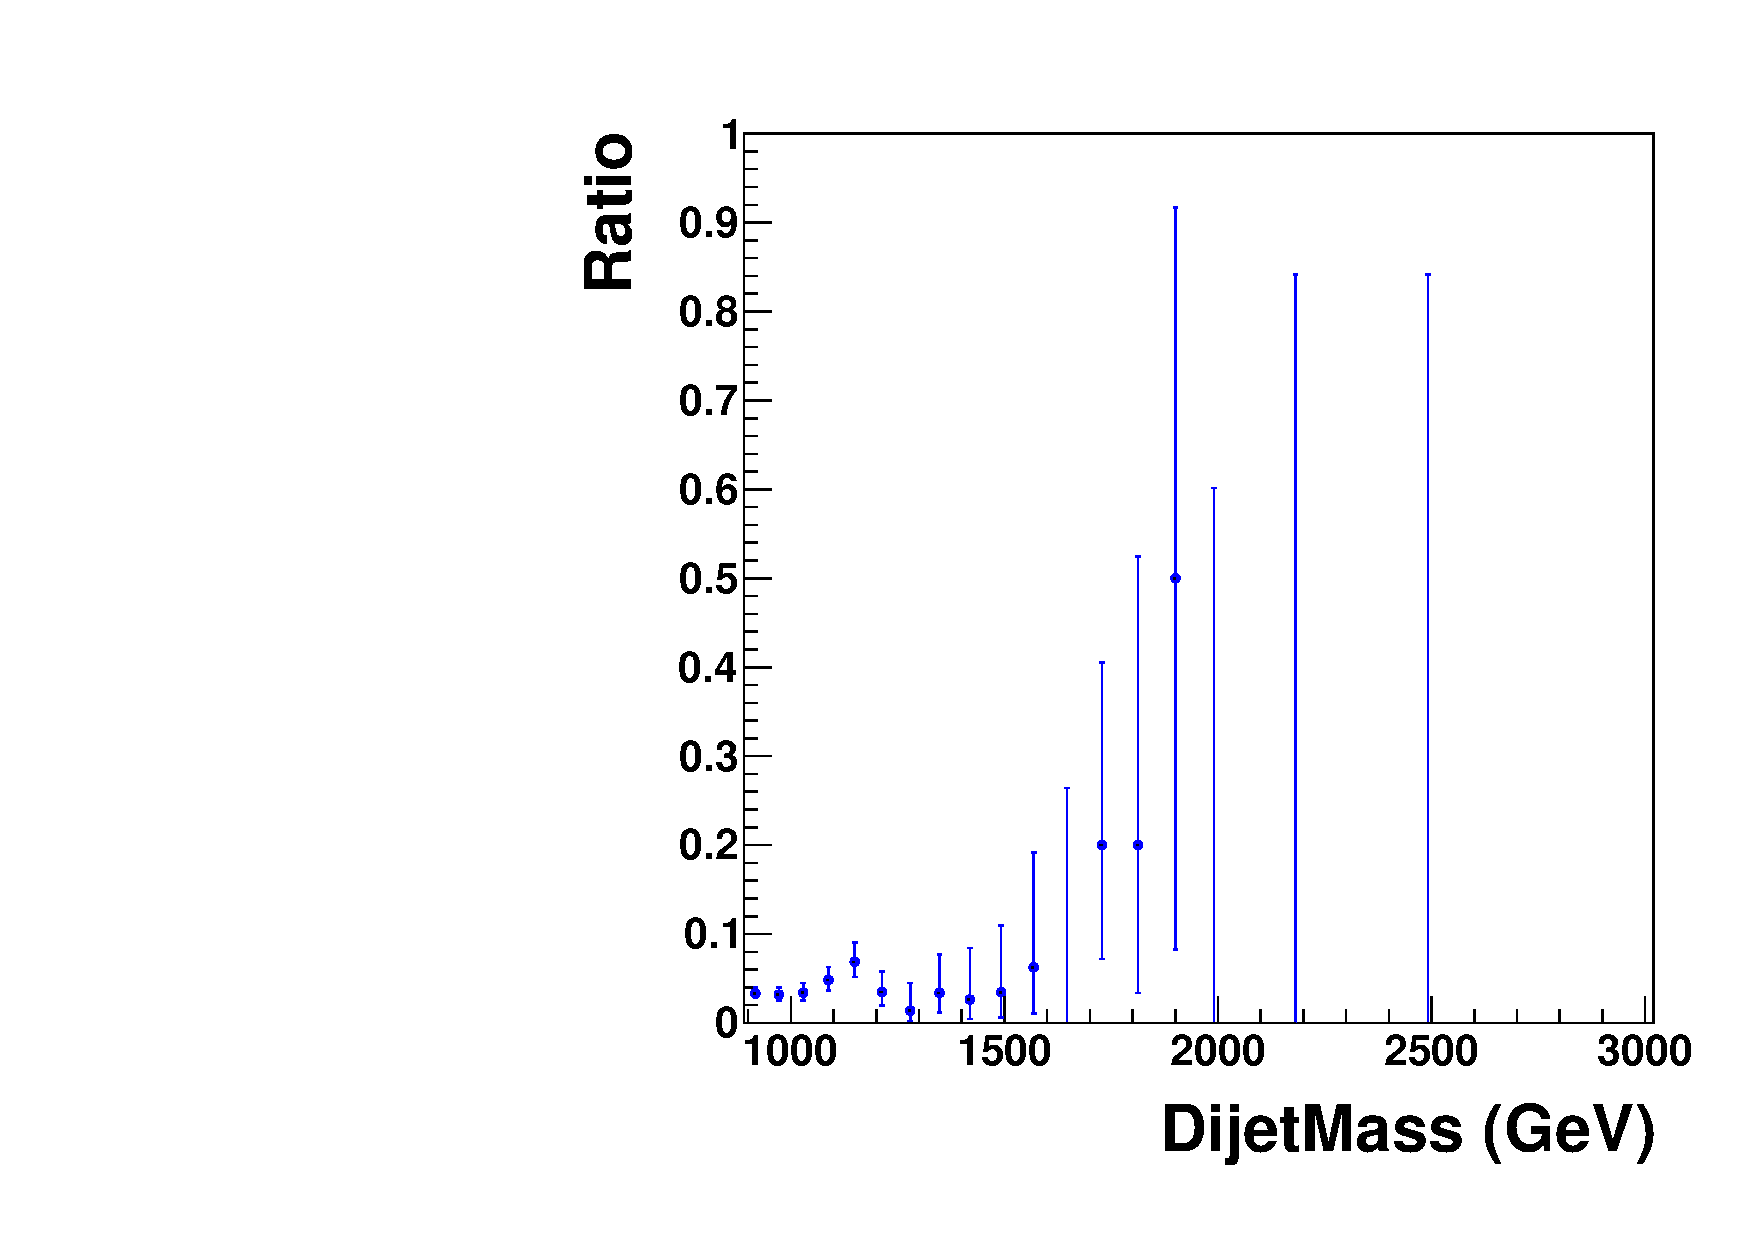
\includegraphics[width=0.49\textwidth]{HqqqqZqqfigs/HbbHww/HighPurityRatio.pdf}
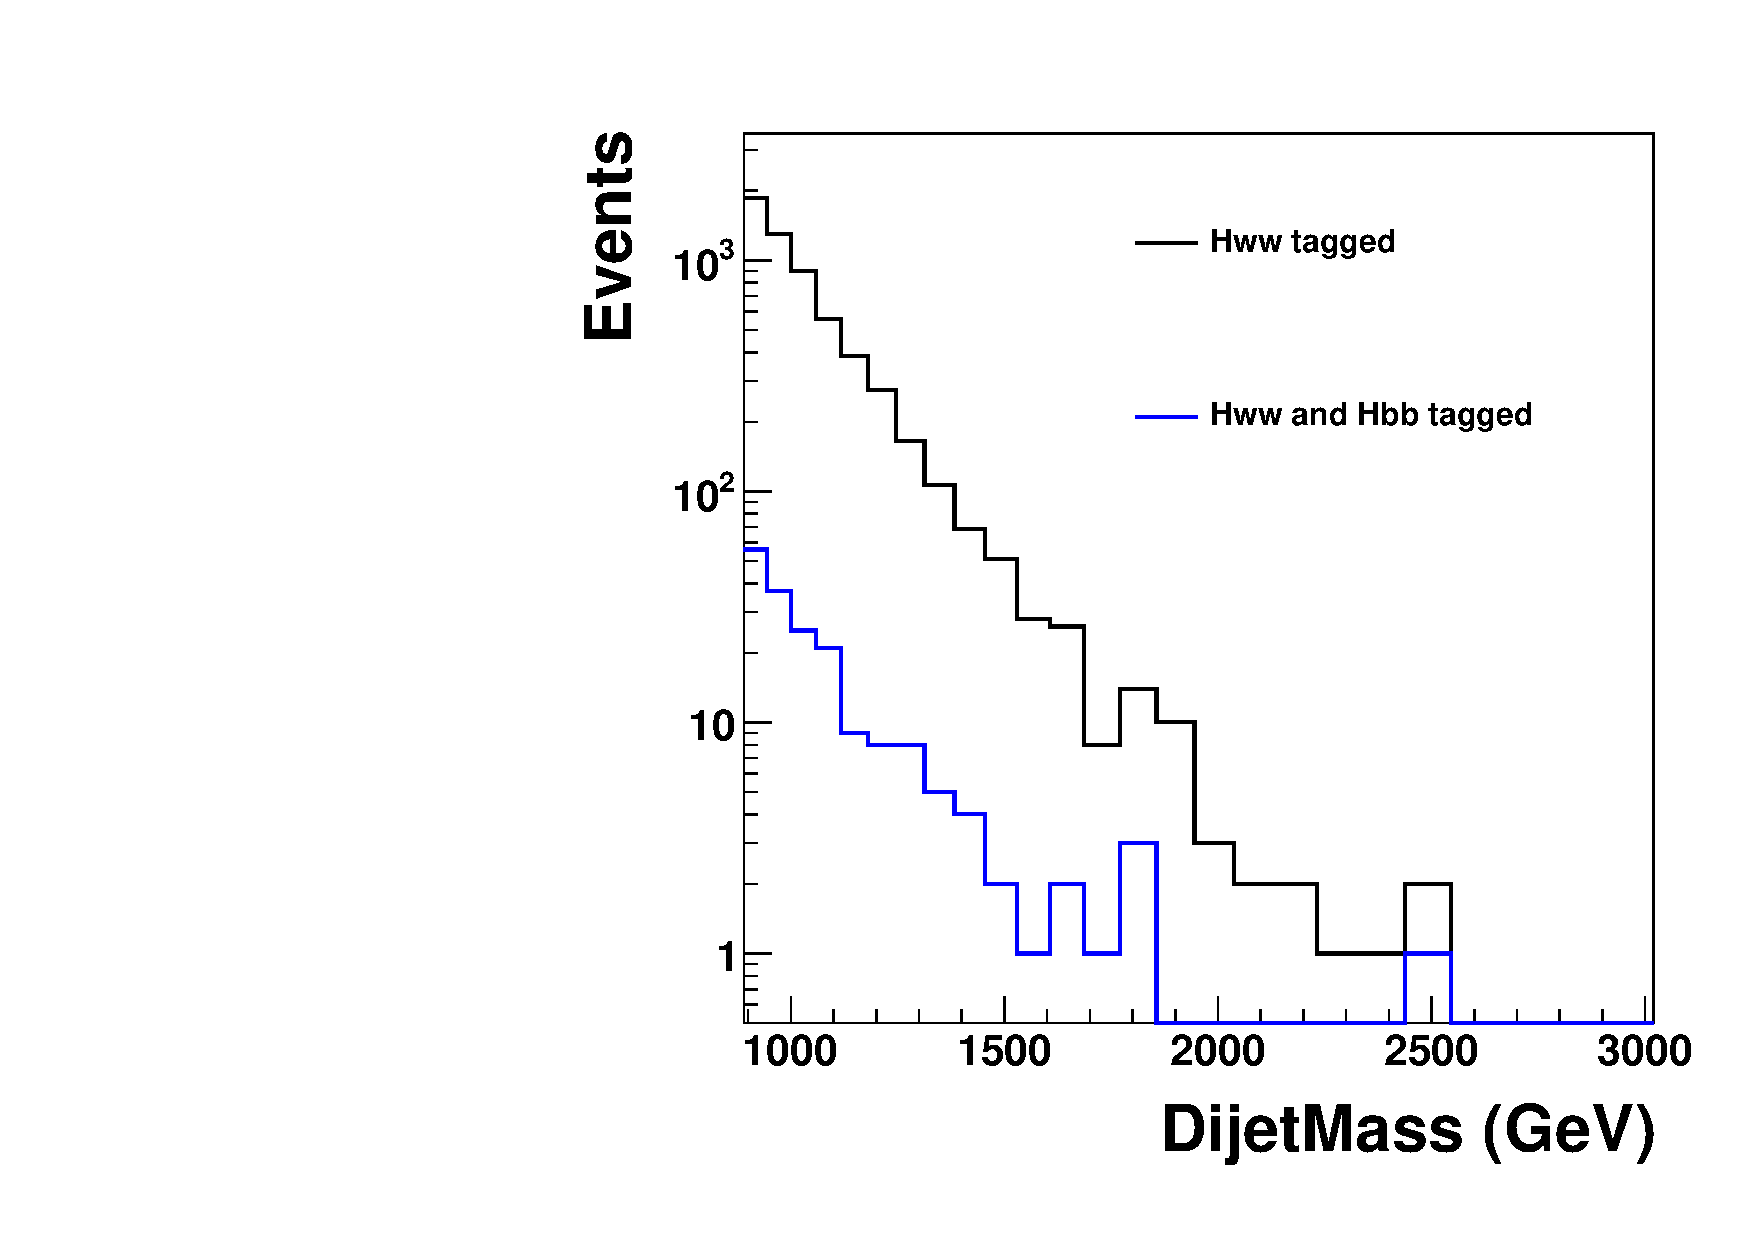
\includegraphics[width=0.49\textwidth]{HqqqqZqqfigs/HbbHww/LowHPurity.pdf}
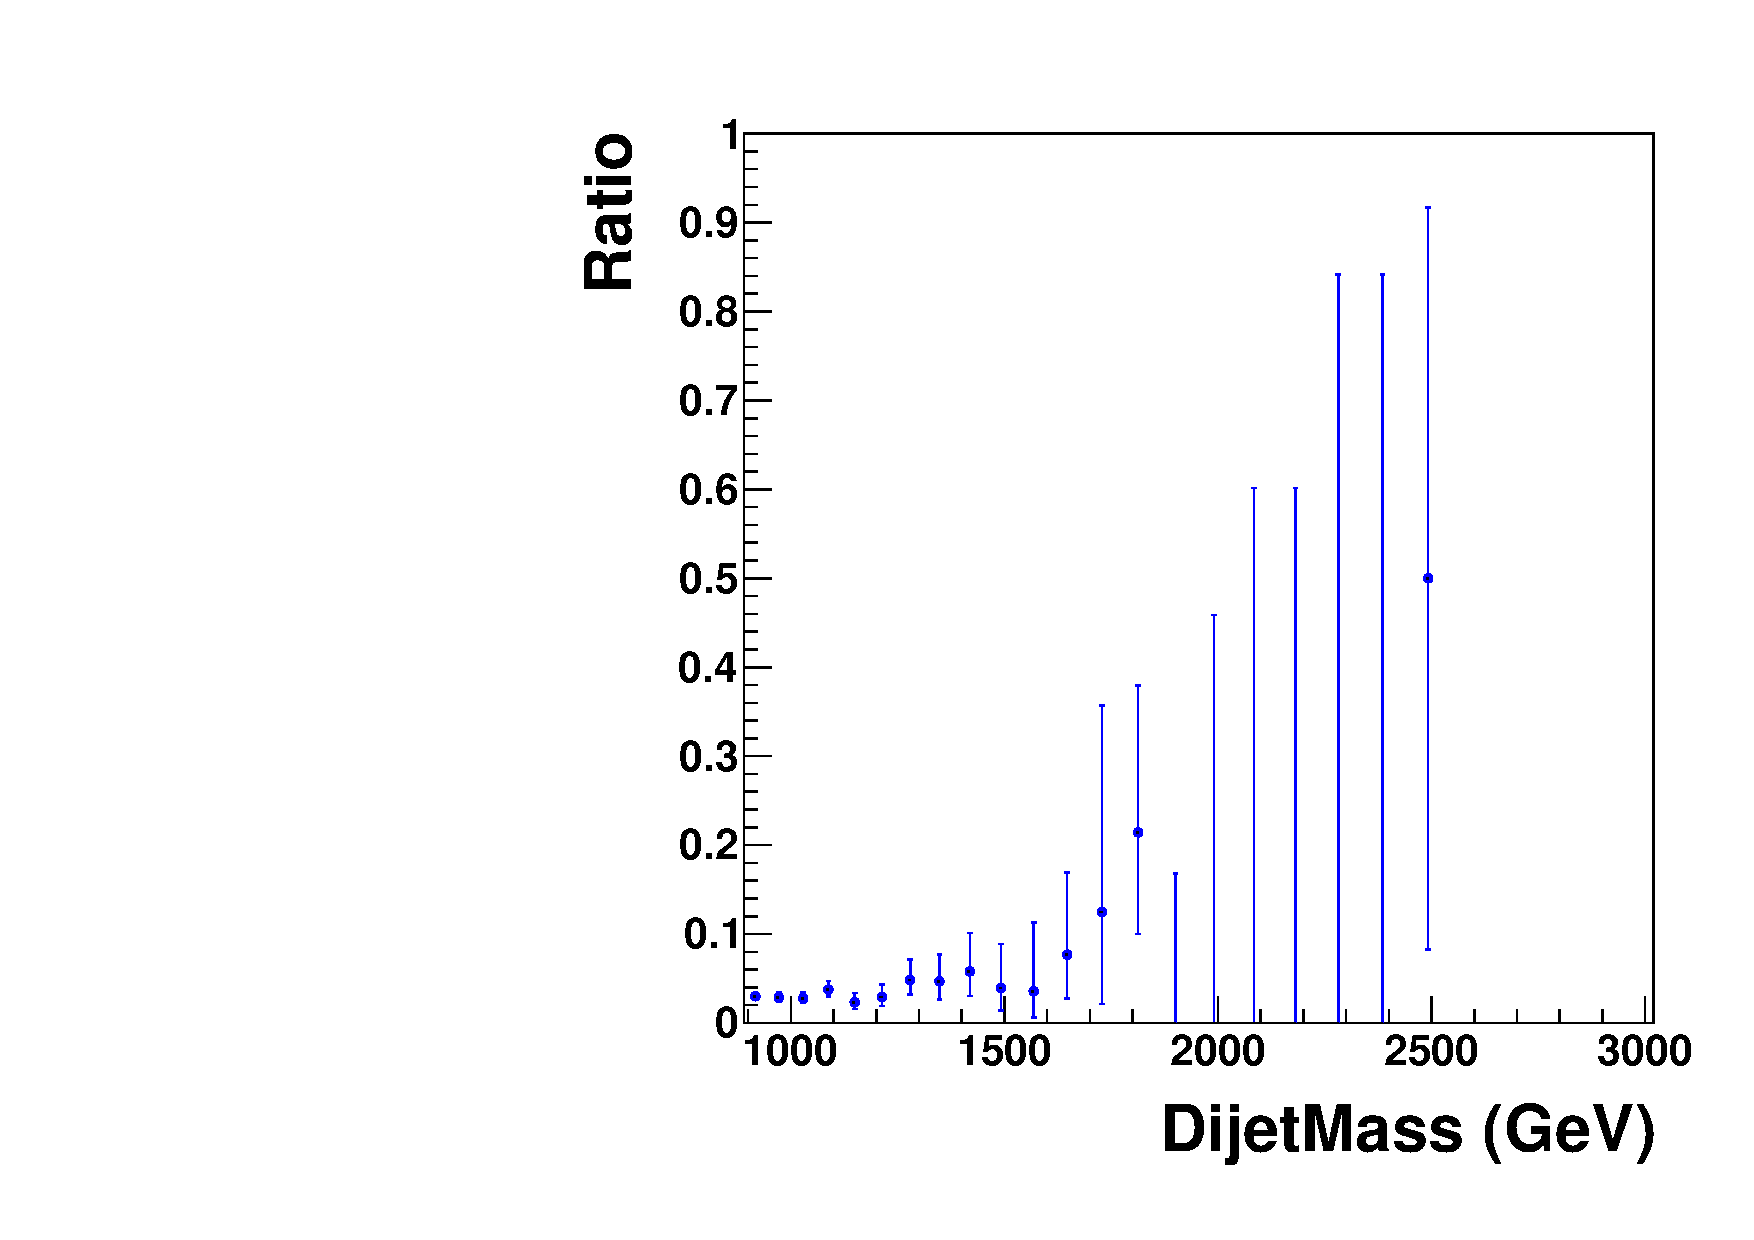
\includegraphics[width=0.49\textwidth]{HqqqqZqqfigs/HbbHww/LowHPurityRatio.pdf}
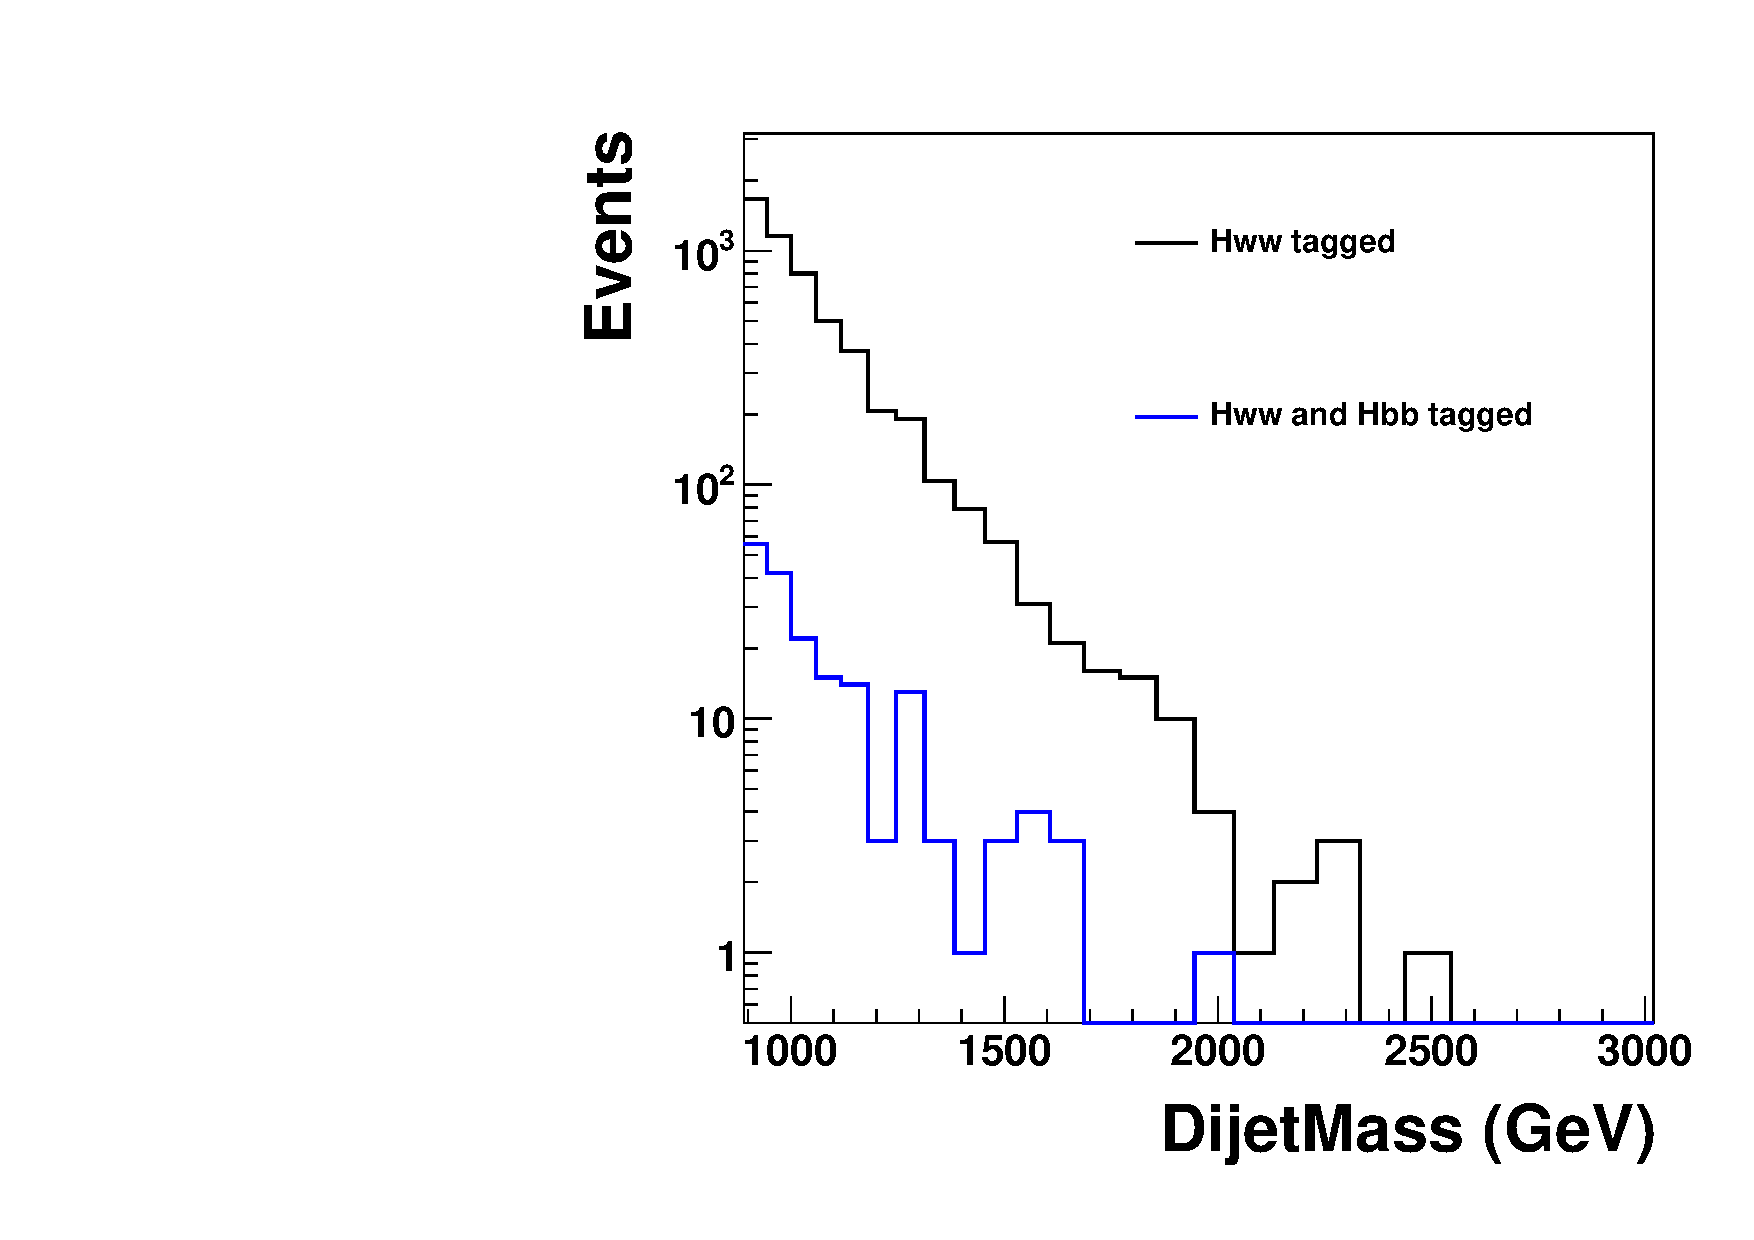
\includegraphics[width=0.49\textwidth]{HqqqqZqqfigs/HbbHww/LowVPurity.pdf}
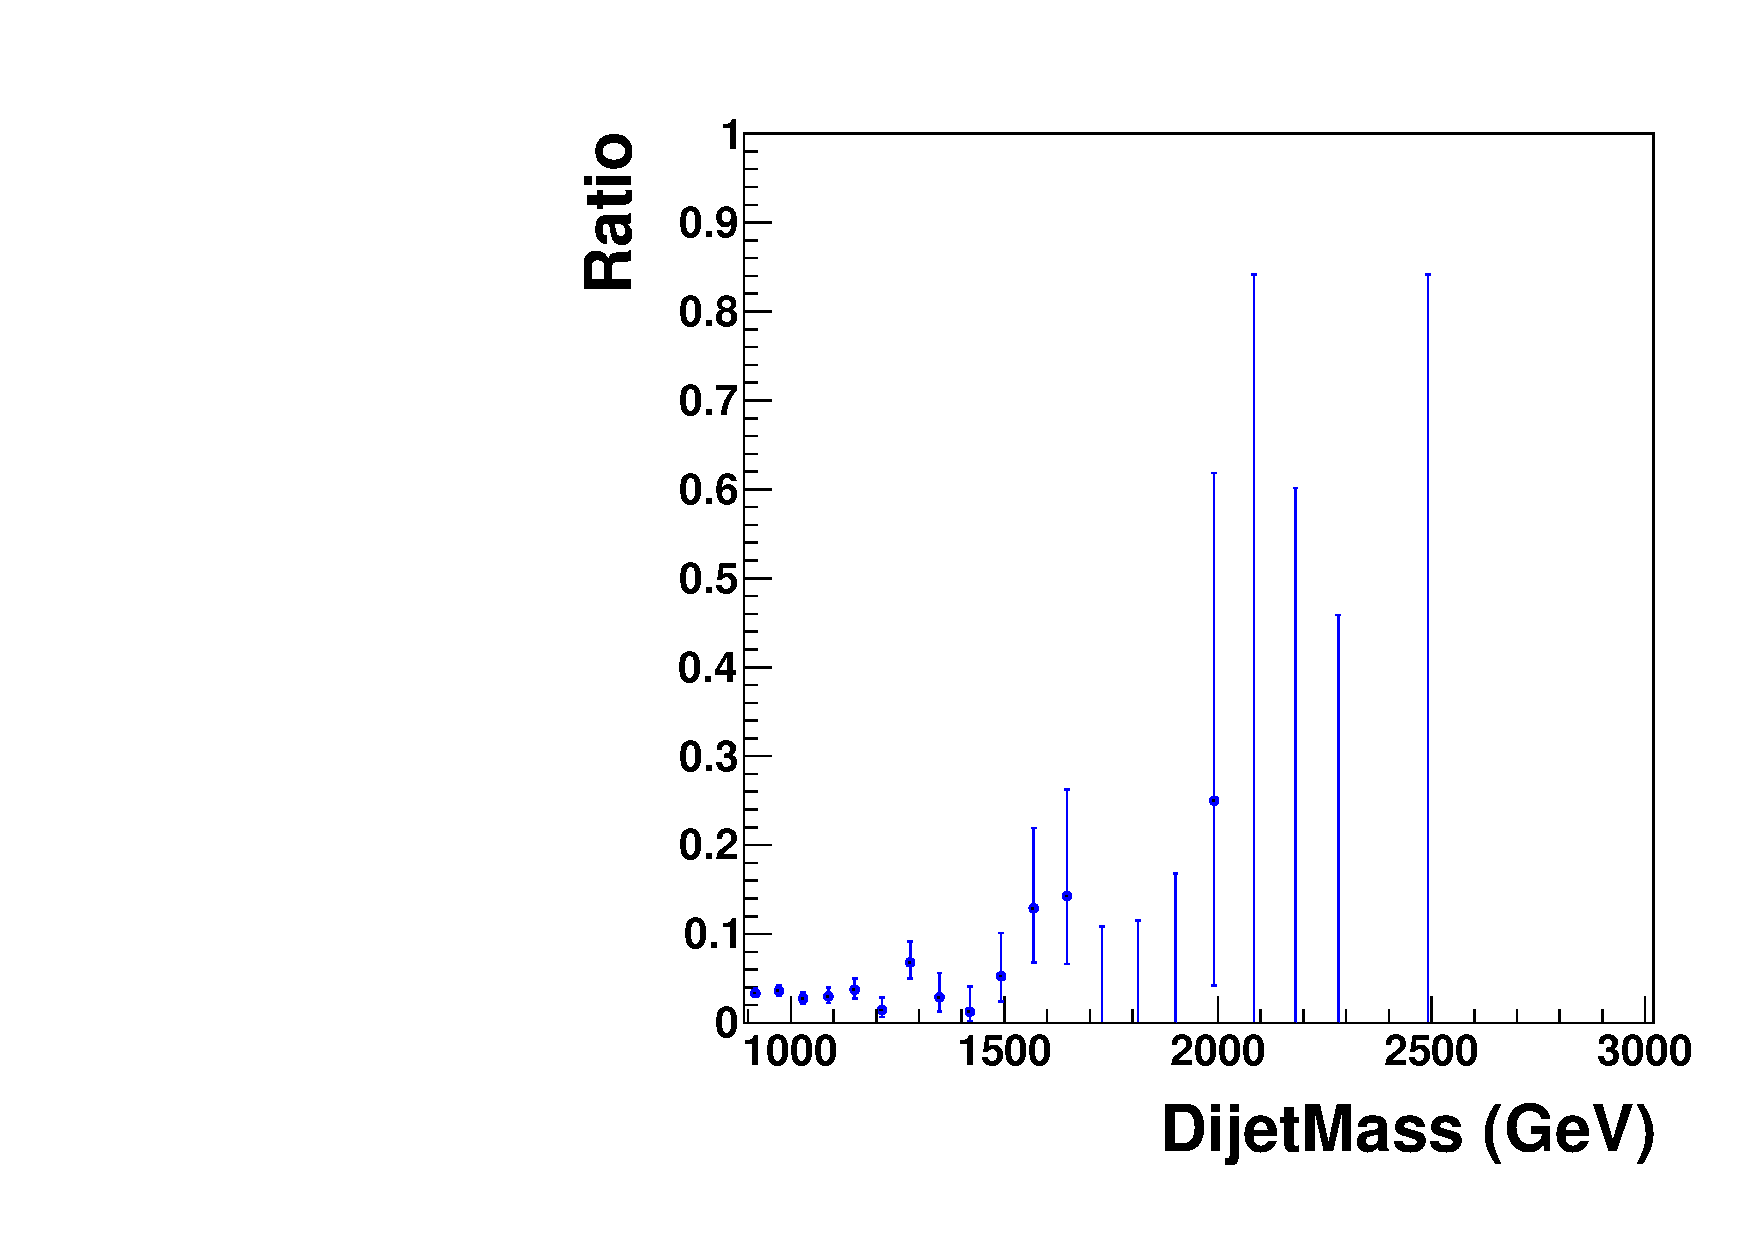
\includegraphics[width=0.49\textwidth]{HqqqqZqqfigs/HbbHww/LowVPurityRatio.pdf}
\end{center}
\caption{
Dijet mass distribution in data, for events pass Hww tagger only. And evnts pass both Hww and Hbb tagger.Plot on the top right, is the High purity Hww tagger, plots in the middle are the Low purity Hww tagger. Plots on the bottom are the low purity V tagger.  Plots on 
the right hand are the corresponding ratio(#EventsPassHbbHww/#EventsPassHww) plot.  
}
\label{fig:HbbRatio}
\end{figure}

\clearpage

